\documentclass[headings=standardclasses,headings=big,oneside,a4paper,openany,12pt]{scrbook}

\newcommand {\e}[1]{\mathrm{~#1}}
\newcommand {\E}[1]{\times 10^{#1}}
\newcommand {\vars}{$\Delta E$ and $M_{BC}$}
\newcommand {\btbii}{\texttt{B2BII}}
\newcommand {\decaya}{$B \to K K \ell \nu$}
\newcommand {\decayb}{$B^+ \to K^+ K^- \ell^+ \nu$}

%\usepackage{biblatex}
%\bibliography{mybib.bib} 
\usepackage[slovene,english]{babel}% Recommended
\usepackage{csquotes}% Recommended
\usepackage[sorting=none,firstinits=true,backend=bibtex]{biblatex}
\addbibresource{mybib.bib}% Syntax for version >= 1.2

\usepackage{paralist}
\usepackage{caption}
\usepackage{cancel}

\usepackage{longtable}

\setlength{\parskip}{1em}%
\setlength{\parindent}{0cm}

\usepackage{titling}
\usepackage{amsmath,amssymb,amsfonts,nicefrac}
\usepackage{graphicx}
\usepackage{color}
\usepackage{float}
\usepackage{mathtools}
\allowdisplaybreaks
\usepackage[pdftex,colorlinks=true,citecolor=blue,linkcolor=black,urlcolor=blue,bookmarks=true]{hyperref}
\usepackage{dictsym}
\usepackage{braket}
\usepackage{slashed}
\DeclareMathOperator{\arcsinh}{arcsinh}
\usepackage{enumerate}
\usepackage{array}
\setlength{\extrarowheight}{.5ex}

\usepackage{lineno}
\linenumbers

\usepackage{subfigure}

\usepackage{titlesec}
\titlespacing*{\subsubsection}
{0pt}{0pt}{0pt}


\begin{document}
\begin{otherlanguage}{slovene}
\chapter{Povzetek doktorskega dela}
\section{Uvod}
Fizika delcev je eden od stebrov fizike, z mo"cnimi koreninami, ki segajo vse do za"cetka 20. stoletja. Natan"cni eksperimenti in preverljiva teorija so pokazali, da vesolje sestoji iz osnovnih delcev in nosilcev interakcij. Osnovne delce delimo na kvarke ($u$, $d$, $s$, $c$, $b$, $t$) in leptone, ki so nadaljnje razdeljeni na nabite leptone ($e$, $\mu$, $\tau$) in pa nevtrine ($\nu_e$, $\nu_\mu$, $\nu_\tau$). Nosilci treh (od "stirih) osnovnih interakcij, s katerimi se ukvarjamo na tem podro"cju, so fotoni ($\gamma$) za elektromagnetno, gluoni ($g$) za mo"cno in nabiti- ($W^\pm$) ter nevtralni ($Z^0$) bozoni za "sibko interakcijo. Vsi delci in njihovi zrcalni partnerji, antidelci (ozna"ceni z $~\bar {}~$), imajo maso, ki jim jo dolo"ca Higgsov bozon ($H$). Vse delce ter interakcije med njimi opisuje Standardni model, ki je osrednja teorije fizike visokih energij. Kvarke lahko zdru"zujemo v kombinacije oblike $q_1 q_2 q_3$ (hadroni) ali pa $q_1 \bar{q}_2$ (mezoni), med katere sodijo tudi protoni in nevtroni, ki jih opazimo v naravi. Poleg omenjenih dolgo-"zive"cih delcev pa obstajajo tudi te"zji, manj stabilni delci, ki preko zgoraj na"stetih interakcij razpadejo v la"zje, stabilnej"se. Raziskovanje tak"snih procesov s pomo"cjo pospe"sevalnikov in trkalnikov nam omogo"ca spoznavanje zakonov vesolja danes pa vse do njegovega za"cetka.

Osrednji del doktorske disertacije predstavljajo meritve razpadov mezonov $B$, delcev, ki so sestavljeni iz te"zkega kvarka $b$ in enega od lahkih kvarkov $u$ ali $d$. Ena bolj presenetljivih lastnosti vesolja je kr"sitev simetrije $CP$, t.j. kombinacije simetrij konjugacije naboja ($C$) in prostorske inverzije ($P$). Simetrija $CP$ nakazuje, da so fizikalni procesi delcev in zrcalni procesi antidelcev enaki, kar pa danes vemo, da ne dr"zi v celoti in poznamo procese, ki to simetrijo kr"sijo. Kr"sitev simetrije $CP$ je tesno povezana s "sibko interakcijo, to pa predstavlja na"so motivacijo za "studijo mezonov $B$, saj "sibki razpadi predstavljajo ve"cji del vseh razpadov mezonov $B$.

Edinstvena lastnost "sibke interakcije je, da lahko spreminja tip oziroma t.i. okus kvarkov, medtem ko ga ostale interakcije ohranjajo. Tak"sni procesi so opisani s prehodno matriko CKM (Cabibbo-Kobayashi-Maskawa) \cite{cabibbo1963unitary,kobayashi1973cp}
\begin{equation}
V_{CKM} = \begin{bmatrix}
    V_{ud} & V_{us} & V_{ub}\\
	V_{cd} & V_{cs} & V_{cb}\\
	V_{td} & V_{ts} & V_{tb}
\end{bmatrix}.
\end{equation}
Unitarnost matrike CKM nam omogo"ca, da iz nje izlu"s"cimo matemati"cne identitete, od katerih je ena pomembnej"sih
\begin{equation}
V_{ud}V_{ub}^* + V_{cd}V_{cb}^* + V_{td}V_{tb}^* = 0,
\end{equation}
poznana pod imenom unitarni trikotnik, saj predstavlja zaklju"cen vektor treh to"ck v kompleksni ravnini, kot prikazuje Slika \ref{fig:ut_si}. Parametri matrike CKM niso dolo"cljivi s strani teorije, temve"c jih moramo dolo"citi z eksperimentalnimi meritvami tako, da najdemo procese, ki so tesno povezani s stranicami in koti unitarnega trikotnika. Na tak na"cin lahko preverimo, "ce je oblika trikotnika konsistentna, kar predstavlja dober test Standardnega modela, oziroma "ce so potencialno prisotni kak"sni novi procesi, ki jih "se ne poznamo, in jih kolektivno imenujemo "nova fizika". Dodatna motivacija za "studijo mezonov $B$ je ta, da velik dele"z njihovih razpadov predstavlja koristne procese za meritev unitarnega trikotnika.
\begin{figure}[H]
\centering
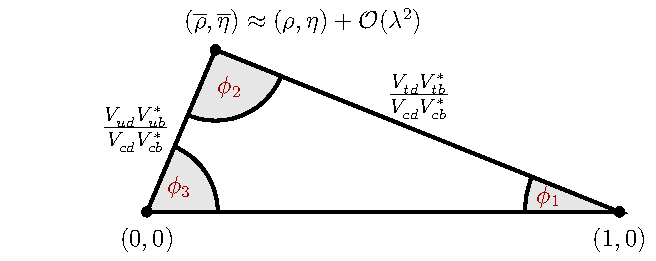
\includegraphics[scale=1]{texfig/UT_Triangle}
\caption{Unitarni trikotnik s parametri $\lambda,~\eta,~\rho$ and $A$ (slednji ni prikazan), ki predstavljajo proste parametre matrike CKM.} %TODO: Wolf. param. 
\label{fig:ut_si}
\end{figure}

Procesi, ki jih "studiramo v tej analizi, so tesno povezani z elementom $V_{ub}$ matrike CKM, saj le-ta opisuje prehode kvarkov $b \to c$. Od vseh elementov, je absolutna vrednost tega elementa najmanj"sa, relativna napaka pa najve"cja, zato meritve iz tega podro"cja potencialno omogo"cajo najve"c izbolj"save. Tak"sni prehodi kvarkov so prisotni v ne"carobnih (t.j. brez kvarkov $c$) semi-leptonskih razpadih mezonov $B$ oblike 
\begin{equation}
B^+ \to X_u^0 \ell^+ \nu_\ell,
\end{equation}
kjer $X_u^0$ predstavlja ne"carnobne mezone, $\ell$ pa je eden od nabitih leptonov. Frekvenco razpadov, ki je tesno povezana z elementom $V_{ub}$, opi"semo z ena"cbo
\begin{equation}
\mathrm{d} \Gamma \propto G_F^2 \vert V_{ub} \vert ^2 \vert L^\mu \langle X_u \vert \bar u \gamma_u \frac{1}{2} (1-\gamma_5) b \vert B \rangle \vert ^2,
\end{equation}
kjer $G_F$ predstavlja Fermijevo konstanto, $L^\mu$ leptonski tok, izraz v Diracovih oklepajih pa hadronski tok. V tak"snih prehodih $\vert V_{ub} \vert ^2$ predstavlja verjetnost za prehod $b \to u$.

Meritev elementa $V_{ub}$ je mo"zna na ekskluziven in inkluziven na"cin, kjer pri prvi metodi opravljamo meritve v specifi"cno definirana kon"cna stanja, kot na primer $B \to \pi \ell \nu$, pri drugi metodi pa opravljamo meritev s kupno kon"cno stanje oblike $B \to X_u \ell \nu$. Obe metodi potekata preko razli"cnih pristopov in se soo"cata z razli"cnimi tezavami, kar pomeni, da sta oba kon"cna rezultata nekorelirana. Rezultata obeh meritev imata tudi zelo podobno natan"cnost, medtem ko se srednja vrednost le deloma ujema. Rezultata se razlikujeta s signifikanco $3\sigma$, kar predstavlja ve"cjo te"zavo znotraj podro"cja. Trenutni svetovni povpre"cji \cite{Amhis:2016xyh} ekskluzivne (iz razpadov $B^0 \to \pi^- \ell^+ \nu$) in inkluzivne meritve (GGOU kolaboracija \cite{Gambino:2007rp}) sta
\begin{align}
&\vert V_{ub} \vert_{\mathrm{e.}} = \left(3.65 \pm 0.09 \pm 0.11\right)\E{-3},\\
&\vert V_{ub} \vert_{\mathrm{i.}}^{\mathrm{GGOU}} = \left(4.52 \pm 0.15~{}^{+0.11}_{-0.14}\right)\E{-3},
\end{align}
kjer prva in druga napaka predstavljata eksperimentalno in teoretsko napako. Rezultati inkluzivnih meritev so praviloma ve"cji kot rezultati ekskluzivnih. Razlogov za neujemanje je lahko ve"c, od nepoznanih napak pri eksperimentu ali teoriji, do prispevkov nove fizike.

V tej analizi se osredoto"camo na enega od mo"znih razlogov za zgoraj omenjeno neujemanje, konkretneje za razpad \decayb, ki je strukturno precej podoben razpadu $B \to \pi \ell \nu$ za razliko produkcije para kvarkov $s \bar s$ ki se potem hadronizira v nove delce, kot prikazuje Slika \ref{feynman}. V inkluzivnih meritvah ne"carobnih semi-leptonskih razpadov mezonov $B$ se standardno uporablja $K$-veto, t.j. selekcija, kjer zahtevamo, da v kon"cnem stanju nimamo mezonov $K$ (sestava $q \bar s,~q \in [u,d]$), poznanih tudi pod imenom kaoni. Kaoni v kon"cnem stanju nakazujejo na pogost prehod kvarkov $b \to c \to s$, ki pa jih ho"cemo v analizah prehodov $b \to u$ zatreti. V primeru na"se analize imamo v kon"cnem stanju 2 kaona s prehodom $b \to u$, kar pomeni, da tak"sni razpadi niso upo"stevani v inkluzivnih meritvah, "ceprav bi morali biti. Cilj "studije je dolo"citi pogostost razpadov \decayb~s prehodom $b\to u$ in s tem oceniti, kak"sen potencialen efekt ima lahko neupo"stevanje teh razpadov na inkluzivno meritev elementa $V_{ub}$. V nadaljevanju bo razpad \decayb~zaradi enostavnosti zapisan kot \decaya.
\begin{figure}[H]
\centering
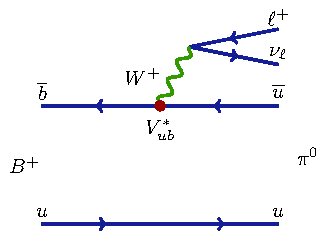
\includegraphics{texfig/B2pilnu}
\hspace{1cm}
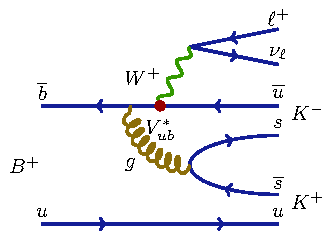
\includegraphics{texfig/B2KKlnu}
\caption{Feynmanovi diagrami za razpada $B^+ \to \pi^0 \ell^+ \nu_\ell$ (levo) in $B^+ \to K^- K^+ \ell^+ \nu_\ell$ (desno).}
\label{feynman}
\end{figure}

\section{Experimentalna postavitev}

Podatki, uporabljeni v tej analizi, so bili ustvarjeni pri trkih elektronov $e^-$ in pozitronov $e^+$ v pospe"sevalniku KEKB in zajeti z detektorjem Belle. Eksperiment je trajal od leta 1999 do 2010 pod okriljem znanstvene organizacije KEK v mestu Tsukuba na Japonskem. Trki delcev so se dogajali pri energiji, ki je ustrezala masi resonance $\Upsilon(4S)$, (sestava $b \bar b$). V tem delu disertacije sta opisana pospe"sevalnik in detektor, podrobnej"si opis pa se nahaja v literaturah \cite{doi:10.1093/ptep/pts102} in \cite{ABASHIAN2002117}.

\subsection{Trkalnik KEKB}

KEKB je asimetri"cen trkalnik delcev $e^+e^-$, ki potujejo po obro"cih s premerom $3\e{km}$ v gru"cah. V sredi"s"cu detektorja gru"ci elektronov z energijo $8\e{GeV}$ in pozitronov z energijo $3.5\e{GeV}$ tr"cita pod kotom $22\e{mrad}$. Skupna invariantna masa trka ustreza masi resonance $\Upsilon(4S)$ 
\begin{equation}
E_{CM} = 2\sqrt{E_{e^+}E_{e^-}} = m_{\Upsilon(4S)}c^2 \approx 10.58\e{GeV}.
\end{equation}
Dele"z mezonov $\Upsilon(4S)$ razpade preko zelo "cistega kanala v dva prakti"cno mirujo"ca mezona $B$, kar tej in v podobnih analizah pogosto izkori"s"camo, saj je za"cetno stanje dobro poznano.

Trkalnik je v "casu obratovanja zajel koli"cino podatkov, ki ustreza integrirani luminoznosti $1041\e{fb^{-1}}$, od katere okoli $711\e{fb^{-1}}$ predstavlja podatke, zajete pri energiji $10.58\e{GeV}$, t.j. masi resonance $\Upsilon(4S)$. Slednja vrednost integrirane luminoznosti ustreza "stevilu $771\E{6}$ parov $B \bar B$ mezonov.

\subsection{Detektor Belle}
Detektor Belle je magnetni masni spektrometer, ki pokriva ve"cji del prostorskega kota. Njegov namen je, da detektira delce, ki se gibljejo v magnetnem polju $1.5\e{T}$ in so potomci trkov $e^+e^-$. Cilj je dolo"citi energijo in gibalno koli"cino delcev, kar dose"zemo preko detektorskih podsistemov, ki so okoli interacijske to"cke postavljeni v plasteh. Detektor pokriva polarni kot med $17^\circ \leq \theta \leq 150^\circ$, med tem ko je azimutni kot pokrit v celoti, kar skupaj predstavlja $92\%$ pokritost polnega prostorskega kota.
\subsubsection{Silikonski  detektor verteksov}
Silikonski detektor verteksov je postavljen najbli|zje interakcijski to"cki. Sestavljen je iz dvostranskih silikonskih detektorjev, ki podajajo 2D informacijo o prehodih nabitih delcev z natan"cnostjo okoli $100\e{\mu m}$. To nam omogo"ca dolo"citev to"ck razpada (verteksov) kratko-"zivecih delcev.

\subsubsection{Osrednja potovalna komora}
Osrednja potovalna komora je sestavljena iz mnogo "zic, napeljanih skozi me"sanico plina.  Komora tako meri sledi nabitih delcev, ki potujejo skozi magnetno polje v detektorju. Preko sledi lahko dolo"cimo informacijo o gibalni koli"cini delca, hkrati pa v obmo"cju gibalne koli"cine pod $0.8\e{GeV}/c$ slu"zi tudi za njihovo identifikacijo.

\subsubsection{Merilec "casa preleta}
Merilec "casa preleta meri "casovno razliko od trka pa do preleta delca skozi enega od scintilatorjev tega podsistema. Namen je identifikacija delcev v obmo"cju gibalnih koli"cin $0.8\e{GeV}/c < p < 1.2\e{GeV}/c$, "se posebej kaonov $K^\pm$ in pionov $\pi^\pm$. Pri isti gibalni koli"cini zaradi razli"cnih mas delcev dobimo razli"cne case preleta, kar lahko uporabimo za dolo"citev njihove mase. "Casovna resolucijo tega podsistema je bolj"sa kot ali enaka $100\e{ps}$.

\subsubsection{Pragovni "stevec sevanja "Cerenkova}
"Stevec sevanja "Cerenkova se prav tako uporablja za identifikacijo delcev, deluje pa v vi"sjih obmo"cjih gibalne koli"cine, kjer merilec "casa preleta ni ve"c zadosten, t.j. v obmo"cju $1.0\e{GeV}/c < 4.0\e{GeV}/c$. Silikatni aerogel z dobro dolo"cenim lomnim koli"cnikom predstavlja osrednjo strukturo podsistema, seva "Cerenkovo svetlobo, "ce ga preletijo delci, ki se gibljejo hitreje od svetlobne hitrosti v tej snovi. Pragovni "stevec deluje na osnovi, da prelet la"zjih delcev povzro"ci sevanje "Cerenkova, prelet te"zjih delcev pa ne.

\subsubsection{Elektromagnetni kalorimeter}
Elektromagnetni kalorimeter slu"zi za detekcijo delcev, ki interagirajo elektromagnetno, predvsem elektronov in fotonov. Z njim lahko izmerimo pozicijo in energijo delca, ko zadane kalorimeter. Ko elektroni ali fotoni zadanejo kristalne celice kalorimetra, povzro"cijo t.i. elektromagnetni tu"s, medtem ko drugi, te"zji delci, ne interagirajo na enak na"cin in v kalorimetru pustijo le majhen dele"z energije. Energijska lo"cljivost kalorimetra je pribli"zno $1.7\%$.

\subsubsection{Detektor mezonov $K_L^0$ in mionov}
Za elektromagnetnim kalorimetrom, na drugi strani magnetnega jedra, je postavljen detektor mezonov $K_L^0$ in mionov za gibalno koli"cino ve"cjo od $0.6\e{GeV}/c$. Ti delci so so visoko penetrirajo"ci, saj lahko preletijo vse do sedaj opisane podsisteme. Prvi so nevtralni in jih lahko dolo"cimo preko hadronske interakcije v detektorju in preko manjkajo"ce nabite sledi, medtem ko so drugi nabiti in jih identificiramo "ze samo z njihovo prisotnostjo.

\section{Analizni postopek}
Analizni postopek je določen na podlagi simuliranih podatkov, oziroma Monte Carlo (MC) simulacije. Ta nam omogoča, da na podlagi teoretičnega modela razpadov, dobro opišemo realnost, dodatno pa nam je na voljo "resnica", kot na primer generirane lastnosti delcev in njihova identiteta, ki je bila določena ob generaciji.

Za pripravo analiznega postopka imamo na voljo $6-10\times$ več podatkov kot jih je izmerjenih, s čimer povečamo natančnost analiznih korakov in zmanjšamo možnost statističnih fluktuacij.

Poleg signalnega razpada \decayb, v študiji rekonstruiramo tudi t.i. kontrolni razpad $B^+ \to \bar D {}^0 \ell^+ \nu,~\bar D{}^0 \to K^+K^-$. Drugi ima enako končno stanje kot prvi, le da se zgodi pri prehodu kvarkov $b \to c$, za razliko prehoda $b \to u$ pri prvem razpadu. Ločimo jih lahko zelo dobro preko invariantne mase dveh kaonov, ki je v primeru kontrolnega razpada zelo omejena okoli mase mezona $D^0$, v primeru signalnega razpada pa je razporejena po celotnem območju, kot prikazuje Slika X.

PLOT

\subsection{Rekonstrukcija razpada}

Postopek rekonstrukcije pričnemo z izbiro dolgo-živečih stabilnih delcev, ki so v našem primeru elektroni $e^\pm$, mioni $\mu^\pm$ ter kaoni $K^\pm$. Vsi so nabiti in v detektorju pustijo sled. Nevtrino $\nu$ je nevtralen in interagira le preko šibke interakcije, zato jih s takšnim detektorjem ne moremo opaziti, kar predstavlja manjkajočo energijo in gibalno količino v dogodku trka $e^+e^-$.

Selekcija poteka na podlagi reza spremenljivk, kjer je izbrano območje določeno na podlagi optimizacije metrike FOM (ang. \textit{figure of merit}), definirane kot 
\begin{equation}
FOM = \frac{N_S}{\sqrt{N_S + N_O}},
\end{equation}
kjer $N_S$ predstavlja pravilno rekonstruirane kandidate (signal), $N_O$ pa nepravilno rekonstruirane (ozadje).

Povzeta selekcija dolgo-živečih stabilnih delcev je
\begin{itemize}
\item elektroni: $\vert d_0 \vert < 0.1\e{cm},~\vert z_0 \vert < 1.5\e{cm},~p_{CMS} \in [0.4,\,2.6]~\e{GeV}/c,~PID_e > 0.9$,
\item mioni: $\vert d_0 \vert < 0.1\e{cm},~\vert z_0 \vert < 1.5\e{cm},~p_{CMS} \in [0.6,\,2.6]~\e{GeV}/c,~PID_\mu > 0.97$,
\item kaoni: $\vert d_0 \vert < 0.15\e{cm},~\vert z_0 \vert < 1.5\e{cm},~p_{CMS} \in [0,\,2.5]~\e{GeV}/c,~PID_{K/\pi} > 0.6$,
\end{itemize}
kjer $d_0$ in $z_0$ predstavljata vpadne parametre nabitih delcev, $p_{CMS}$ gibalno količino v težiščnem koordinatnem sistemu, $PID_e$ in $PID_\mu$ metriko identifikacije delcev za elektrone in mione, $PID_{K/\pi}$ pa metriko separacije med kaoni in pioni.

Iz izbranih kandidatov nato naredimo kombinacije $Y = KKe,~KK\mu$, ki služijo kot kandidati mezonov $B$, z izjemo manjkajočih nevtrinov. Na podlagi dejstva, da je detektor Belle hermetično zaprt in pokriva večino prostorskega kota, in da dobro poznamo začetno stanje $\Upsilon(4S)$, lahko določimo četverec manjkajoče (ang. \textit{missing}) gibalne količine kot
\begin{align}
\mathrm{p}_{miss} &= \mathrm{p}_{\Upsilon(4S)} - \sum_i^{\mathrm{Dogodek}}\left(E_i,\,\vec{p}_i \right),\\
\label{eq:ROEloop_si}
\mathrm{p}_{miss} &= \mathrm{p}_{\Upsilon(4S)} - \left(\mathrm{p}_{Y} -\sum_i^{\mathrm{ROE}}\left(E_i,\,\vec{p}_i \right)\right),
\end{align}
kjer $\mathrm{p}$ predstavlja četverec gibalne količine, indeks $i$ teče po vseh delcih znotraj množice, ROE (ang. \textit{rest of event}) pa predstavlja podmnožico celotnega dogodka, ki vsebuje vse delce, ki niso bili uporabljeni v rekonstrukciji kandidata $Y$.

Tudi na tej stopnji je prisotnih veliko napačnih kombinacij kandidatov $Y$, zato po enakem postopku optimiziramo nadaljnjo selekcijo
\begin{itemize}
\item mezoni $B$: $P(\chi^2,NDF) > 6.0\E{-3}$, $\vert \cos \theta_{BY} \vert < 1.05$, $m_{miss}^2 < 0.975\e{GeV}/c^2$, $5.1\e{GeV}/c^2 < M_{BC} < 5.295\e{GeV}/c^2$, $-1.0\e{GeV} < \Delta E < 1.3\e{GeV},$
\end{itemize}
kjer $P(\chi^2,NDF)$ predstavlja kvaliteto razpadne točke mezona $B$, $m_{miss}^2$ pa invariantno maso četverca manjkajoče gibalne količine v dogodku. Ostali izrazi za $\cos \theta_{BY}$, $M_{BC}$ in $\Delta E$ so
\begin{align}
%TODO fix p in Mbc
\cos \left(\theta_{BY}\right) &= \frac{2E_BE_Y - m_B^2 - m_Y^2}{2\vert \vec{p}_B \vert \vert \vec{p}_Y\vert},\\
M_{BC} &= \sqrt{\left(E_{CMS}/2\right)^2 - \vert \vec{p}_B \vert^2},\\
\Delta E &= E_B - E_{CMS}/2
\end{align}
in po vrsti predstavljajo kot med nominalnim ($B$) in rekonstruiranim ($Y$) mezonom $B$, maso, vezano na energijo žarka v težiščnem koordinatnem sistemu, in razliko energije kandidata in polovice težiščne energije $E_{CMS}$. Za pravilne kombinacije mezonov $B$ ima porazdelitev po $M_{BC}$ vrh pri $m_B$, porazdelitev $\Delta E$ pa okoli $\Delta E \approx 0\e{GeV}.$

Potrebno je omeniti, da so v posameznem dogodku lahko prisotni tako nevtralni kot nabiti delci, ki ne prihajajo neposredno iz trka, temveč so lahko bodisi produkti sekundarnih interakcij v detektorju, bodisi delci, ki izhajajo iz ozadja na račun potovanja žarkov po obročih pospeševalnika. Takšne delce je potrebno odstraniti iz En. (\ref{eq:ROEloop_si}), čemur pravimo "čiščenje dogodka". V tej analizi je bilo opravljeno temeljito čiščenje tako nevtralnih kot nabitih delcev, ki so terjali različne pristope, pri tem pa smo uporabili zelo uspešne metode strojnega učenja za prepoznavanje takšnih neželenih delcev. Slika X prikazuje primerjavo med očiščenim in neočiščenim dogodkom, kjer primerjamo porazdelitvi \vars.

PLOT

\subsection{Odstranjevanje ozadja}

Ozadje v takšni analizi predstavljajo napačni kombinacije razpadne verige signalnega kandidata. Napačna kombinacija lahko pomeni v smislu napačne kombinatorike ali pa končno stanje drugih razpadnih kanalov posnema končno stanje signalnega razpada, z izjemo potencialnih manjkajočih delcev. Takšne kombinacije v splošnem nimajo enakih lastnosti kot signalne kombinacije, zato skušamo najti načine, kako takšno ozadje odstraniti na najbolj optimalen način.

Odstranjevanja ozadja se lotimo v treh korakih, v prvem koraku uporabimo enostavne reze na invariantni masi kaonskega para, saj pričakujemo, da veliko parov $KK$ pride iz resonancam podobnih struktur, kot na primer $\phi \to KK$ ali $D^0 \to KK$, kjer za slednjo že vemo, da je prisotna v kontrolnem razpadu. Prav tako se lahko zgodi, da je eden od pionov napačno identificiran kot kaon. Slika X prikazuje vse reze, ki jih uporabimo za odstranjevanje omenjenih kandidatov, rezi pa so
\begin{itemize}
\item signalni razpad: $\vert m_{KK} - m_{\phi} \vert > \Delta_\phi$, $\vert m_{KK} - m_{D^0} \vert > \Delta_{D^0}$, $\vert m_{K\pi} - m_{D^0} \vert > \Delta_{D^0}$,
\end{itemize}
kjer $m_{KK}$ predstavlja invariantno maso kaonskega para $KK$, $m_{K\pi}$ pa invariantno maso kaonskega para $KK$, kjer je bila masa kaona, katerega naboj je nasproten naboju $B$ mezona, zamenjana z maso delca $\pi^0$. Ostali parametri so $m_\phi \approx 1.019\e{GeV}/c^2$, $m_{D^0} \approx 1.864\e{GeV}/c^2$, $\Delta_\phi \approx 8\E{-3}\e{GeV}/c^2$ in $\Delta_{D^0} \approx 1.5\E{-2}\e{GeV}/c^2$. V primeru študije kontrolnega razpada je bil uporabljen drugačen rez
\begin{itemize}
\item kontrolni razpad: $\vert m_{KK} - m_{D^0} \vert < \Delta_{D^0}$, $\vert m_{K\pi} - m_{D^0} \vert > \Delta_{D^0}$,
\end{itemize}
kjer se osredotočimo na ozko okno okoli mase mezona $D^0$. 

V drugem koraku se lotimo odstranjevanja t.i. kontinuumskega ozadja, kjer kandidati prihajajo iz procesov $e^+e^- \to q \bar q,~q\in[u,d,s,c]$. Poslužimo se metod strojnega učenja, ki prepoznajo kandidate iz kontinuumskih procesov od signalnih kandidatov. Za ta namen potrebujemo spremenljivke, ki opazujejo sferične momente fizikalnih dogodkov, saj so le-ti zelo različni med procesi $e^+e^- \to q \bar q$ in $e^+e^- \to B \bar B$.

V tretjem koraku se na podoben način lotimo odstranjevanja ostalih kandidatov iz procesov $e^+e^- \to B \bar B$, za kar uporabimo vse ostale lastnosti kandidatov, razen \vars, ker le-te potrebujemo za luščenje števila signalnih kandidatov. Pri odstranjevanju ozadja te vrste uporabimo posebno metodo strojnega učenja, ki ohranja obliko porazdelitve spremenljivke $M_{BC}$ za ozadje, kar preprečuje, da bi optimizacija preoblikovala obliko porazdelitve ozadja tisti od signala.

Kot v prejšnjih optimizacijah optimiziramo metriko FOM za odstranjevanje ozadja v drugem in tretjem koraku. Končni vzorec za signalni razpad je prikazan na Sliki X, za kontrolni razpad pa na Sliki X.

PLOT 

PLOT

\subsection{Lu"s"cenje fizikalnih parametrov}

Po selekciji končnega vzorca lahko začnemo luščiti fizikalne parametre iz podatkov.

\subsubsection{Kontrolni razpad}

\subsubsection{Signalni razpad}

\section{Sistematske negotovosti}

\section{Kon\v cni rezultat}

\end{otherlanguage}
\end{document}


